\documentclass{article}

%若使用中文,使用xeLatex编译,并使用XeCJK宏包
\usepackage{xeCJK}


% if you need to pass options to natbib, use, e.g.:
%     \PassOptionsToPackage{numbers, compress}{natbib}
% before loading neurips_2018

\usepackage[final]{neurips_2018}

% to avoid loading the natbib package, add option nonatbib:
%     \usepackage[nonatbib]{neurips_2018}

\usepackage[utf8]{inputenc} % allow utf-8 input
\usepackage[T1]{fontenc}    % use 8-bit T1 fonts
\usepackage{hyperref}       % hyperlinks
\usepackage{url}            % simple URL typesetting
\usepackage{booktabs}       % professional-quality tables
\usepackage{tikz}
\usepackage{amsfonts}       % blackboard math symbols
\usepackage{nicefrac}       % compact symbols for 1/2, etc.
\usepackage{microtype}      % microtypography
\newfontfamily\urlfontfamily{FandolSong-Regular}
\def\UrlFont{\urlfontfamily}

\title{2018-2019学年第二学期COMP130137.01\\
《模式识别与机器学习》课程项目\\
2019语言与智能技术竞赛-机器阅读理解}

\author{\\
学号:xxxxxx , 姓名:xxxxxx,贡献: xx\%,签名:}

\begin{document}
\begin{center}
  声明:我已知悉学校对于考试纪律的严肃规定,将秉持诚实守信宗旨,严守考试纪律,不作弊,不剽窃;若有违反学校考试纪律的行为,自愿接受学校严肃处理。
\end{center}
\maketitle

\begin{abstract}
   Abstract
\end{abstract}

\section{Overview}
\subsection{Introduction}
Machine Reading Comprehension (MRC) means that let machine read context and then answer the question which is based on the material. MRC is an important frontier in the field of natural language processing and artificial intelligence. The competition focus on the problem which are hard to answer in 2018 Machine Reading Comprehension Technology Competition.
\subsection{Assignment}
For a given question \emph{q} and its corresponding text form candidate document set \emph{D = d1, d2, ..., dn}, the participation reading comprehension system is required to automatically analyze the problem and the candidate document, and output a text answer \emph{a} that satisfies the question. The goal is that \emph{a} can answer the question \emph{q} correctly, completely, and concisely.
\subsection{About Dataset}
The dataset contains about 280,000 real problem from Baidu Research, and each of them correspond to 5 candidate document and manual answer. The data set is divided into a training set of 270,000 questions, a development set of approximately 3,000 question, and a test set of approximately 7,000 questions.

\section{BERT and BiDAF Introduction}
\subsection{BERT}
BERT, which stands for Bidirectional Encoder Representations from Transformers, is a new language representation model. BERT is designed to pre-train deep bidirectional representations from unlabeled text by jointly conditioning on both left and right context in all layers. As a result, the pre-trained BERT model can be finetuned with just one additional output layer to create state-of-the-art models for a wide range of tasks, without substantial task-specific architecture modifications.\citet{DBLP:journals/corr/abs-1810-04805}
\begin{figure}[h]
	\centering
	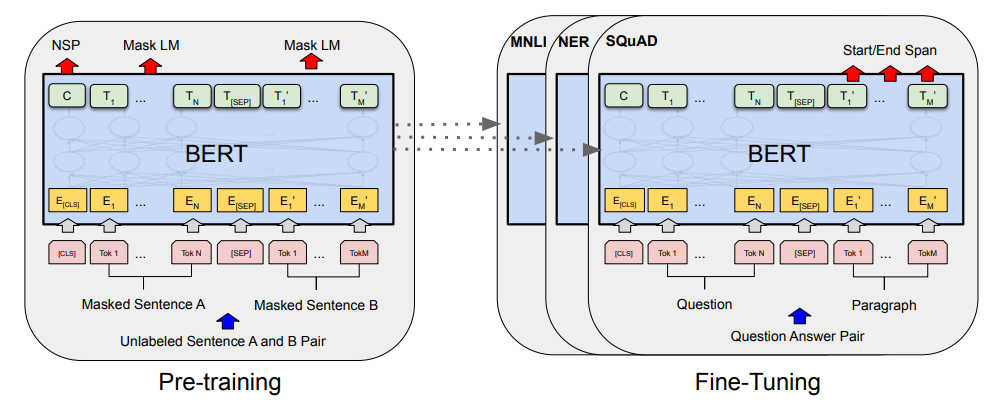
\includegraphics[scale=0.4]{bert.png}
	\caption{Overall pre-training and fine-tuning procedures for BERT}
\end{figure}

\subsection{BiDAF}
Bi-Directional Attention Flow (BiDAF) network is a hierarchical multi-stage architecture for modeling the representations of the context paragraph as different levels of granularity. BIDAF includes character-level, word-level,  \citet{DBLP:journals/corr/SeoKFH16}
\begin{figure}[h]
	\centering
	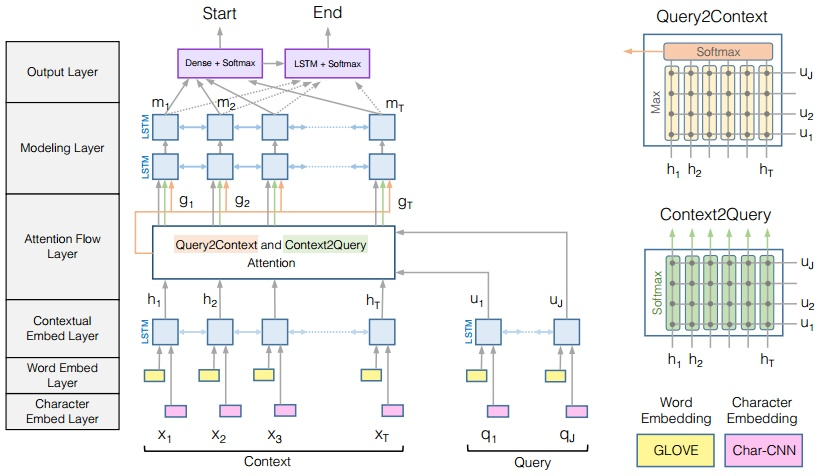
\includegraphics[scale=0.5]{bidaf.jpg}
	\caption{BiDirectional Attention Flow Model}
\end{figure}

\section{Model}
\noindent Our model is a multi-stage process and consists of two parts(Figure 3):\\
\begin{enumerate}
	\item \textbf{BERT} maps each word in query and context to a vector  
	\item \textbf{BiDAF} maps query and context vector in the beginning and ending position of the answer.
\end{enumerate}
\subsection{BERT}
\subsection{BiDAF}
\begin{figure}[h]
	\centering
	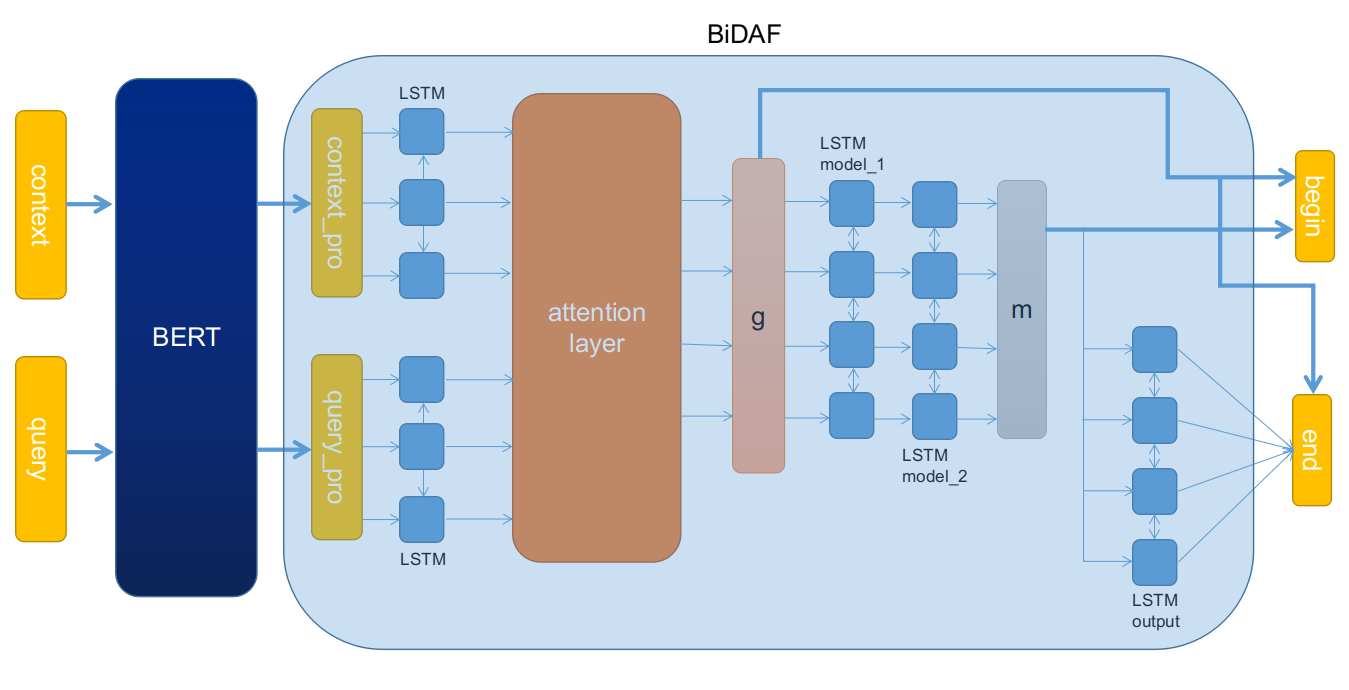
\includegraphics[scale=0.3 ]{Model.png}
	\caption{Model combined by BERT and BiDAF}
\end{figure}
\section{}

选择下面任一项目进行实现。

\subsection{RNN速度改进}
改进LSTM或GRU模型,提高模型并行化能力。

\subsubsection{参考文献}
\begin{enumerate}
    \item Quasi-Recurrent Neural Networks\\ \url{https://openreview.net/forum?id=H1zJ-v5xl}
    \item Simple Recurrent Units for Highly Parallelizable Recurrence\\ \url{https://arxiv.org/abs/1709.02755}
    \item Phased LSTM: Accelerating Recurrent Network
    \item Skip RNN: Learning to Skip State Updates in Recurrent Neural Networks\\ \url{https://openreview.net/forum?id=HkwVAXyCW}
    \item Yu et al., Learning to Skim Text, ACL 2017
    \item Neural Speed Reading via Skim-RNN\\ \url{https://openreview.net/forum?id=Sy-dQG-Rb}
    \item Variable Computation in Recurrent Neural Networks\\
    \url{https://arxiv.org/abs/1611.06188}
\end{enumerate}

\subsection{Few-shot Learning for Text Classification}
Consider a supervised learning task $T$ , FSL deals with a data set $D = \{D_{train},D_{test}\}$ consisting of training set $D_{train} = \{(x^{(i)},y^{(i)})\}^I_{i=1}$ where $I$ is small and test set $D_{test} = \{x_{test}\}$. Usually, people consider the N-way-K-shot classification task  where $D_{train}$ contains $I = KN$ examples
from $N$ classes each with $K$ examples. 

Dataset: \url{https://github.com/Gorov/DiverseFewShot_Amazon}


\subsubsection{参考文献}
\begin{enumerate}
    \item Learning to Compare: Relation Network for Few-Shot Learning\\
    \url{https://arxiv.org/pdf/1711.06025v2.pdf}
    \item A CLOSER LOOK AT FEW-SHOT CLASSIFICATION\\ \url{https://openreview.net/pdf?id=HkxLXnAcFQ}
    \item Advances in few-shot learning: a guided tour\\ \url{https://towardsdatascience.com/advances-in-few-shot-learning-a-guided-tour-36bc10a68b77}
    \item Generalizing from a Few Examples: A Survey on Few-Shot Learning\\
    \url{https://arxiv.org/pdf/1904.05046.pdf}
    \item Advances in few-shot learning: reproducing results in PyTorch\\ \url{https://towardsdatascience.com/advances-in-few-shot-learning-reproducing-results-in-pytorch-aba70dee541d}
    \item  Few-Shot Text Classification with Induction Network\\ \url{https://arxiv.org/pdf/1902.10482.pdf}
\end{enumerate}

\section{实现要求}

项目实现需基于开源项目fastNLP(\url{https://github.com/fastnlp/fastNLP})进行。如果目前的fastNLP功能不足以实现某个算法,可以随便修改。之后也欢迎为fastNLP贡献PR。
具体要求如下:
\begin{enumerate}
    \item 程序正确性,可顺利运行;
    \item 加分项:为fastNLP提PR,并通过单元测试。
    \begin{enumerate}
        \item  GIT操作及PR操作:\url{https://github.com/fastnlp/fastNLP/wiki/怎样使用Git进行开发}
        \item 代码规范参考:\url{https://github.com/fastnlp/fastNLP/wiki/fastNLP-代码规范}
        \item 单元测试说明:\url{https://github.com/fastnlp/fastNLP/wiki/fastNLP测试说明}
    \end{enumerate}
\end{enumerate}


\section{项目报告}
 项目报告作为判断项目质量和工作量的主要依据,请务必详细在报告中描述项目的主要亮点。中英文均可,不少于5页。报告包含以下内容:
\begin{enumerate}
    \item 问题描述、动机
    \item 方法和技术
    \item 实验设计
    \item 结果分析
    \item 相关工作对比、分析
\end{enumerate}


\section{报告的格式信息}
项目报告采用NeurIPS会议论文格式,具体信息如下:

The style files for NeurIPS and other conference information are available on
the World Wide Web at
\begin{center}
  \url{http://www.neurips.cc/}
\end{center}
The file \verb+neurips_2018.pdf+ contains these instructions and illustrates the
various formatting requirements your NeurIPS paper must satisfy.

The formatting instructions contained in these style files are summarized in
Sections \ref{gen_inst}, \ref{headings}, and \ref{others} below.

\section{General formatting instructions}
\label{gen_inst}

The text must be confined within a rectangle 5.5~inches (33~picas) wide and
9~inches (54~picas) long. The left margin is 1.5~inch (9~picas).  Use 10~point
type with a vertical spacing (leading) of 11~points.  Times New Roman is the
preferred typeface throughout, and will be selected for you by default.
Paragraphs are separated by \nicefrac{1}{2}~line space (5.5 points), with no
indentation.


Please pay special attention to the instructions in Section \ref{others}
regarding figures, tables, acknowledgments, and references.

\section{Headings: first level}
\label{headings}

All headings should be lower case (except for first word and proper nouns),
flush left, and bold.

First-level headings should be in 12-point type.

\subsection{Headings: second level}

Second-level headings should be in 10-point type.

\subsubsection{Headings: third level}

Third-level headings should be in 10-point type.

\paragraph{Paragraphs}

There is also a \verb+\paragraph+ command available, which sets the heading in
bold, flush left, and inline with the text, with the heading followed by 1\,em
of space.

\section{Citations, figures, tables, references}
\label{others}

These instructions apply to everyone.

\subsection{Citations within the text}

The \verb+natbib+ package will be loaded for you by default.  Citations may be
author/year or numeric, as long as you maintain internal consistency.  As to the
format of the references themselves, any style is acceptable as long as it is
used consistently.

The documentation for \verb+natbib+ may be found at
\begin{center}
  \url{http://mirrors.ctan.org/macros/latex/contrib/natbib/natnotes.pdf}
\end{center}
Of note is the command \verb+\citet+, which produces citations appropriate for
use in inline text.  For example,
\begin{verbatim}
   \citet{adams1995hitchhiker} investigated\dots
\end{verbatim}
produces

  \citet{DBLP:conf/icml/CollobertW08}  investigated\dots


If you wish to load the \verb+natbib+ package with options, you may add the
following before loading the \verb+neurips_2018+ package:
\begin{verbatim}
   \PassOptionsToPackage{options}{natbib}
\end{verbatim}

If \verb+natbib+ clashes with another package you load, you can add the optional
argument \verb+nonatbib+ when loading the style file:
\begin{verbatim}
   \usepackage[nonatbib]{neurips_2018}
\end{verbatim}



\subsection{Footnotes}

Footnotes should be used sparingly.  If you do require a footnote, indicate
footnotes with a number\footnote{Sample of the first footnote.} in the
text. Place the footnotes at the bottom of the page on which they appear.
Precede the footnote with a horizontal rule of 2~inches (12~picas).

Note that footnotes are properly typeset \emph{after} punctuation
marks.\footnote{As in this example.}

\subsection{Figures}

\begin{figure}
  \centering
  \fbox{\rule[-.5cm]{0cm}{4cm} \rule[-.5cm]{4cm}{0cm}}
  \caption{Sample figure caption.}
\end{figure}

All artwork must be neat, clean, and legible. Lines should be dark enough for
purposes of reproduction. The figure number and caption always appear after the
figure. Place one line space before the figure caption and one line space after
the figure. The figure caption should be lower case (except for first word and
proper nouns); figures are numbered consecutively.

You may use color figures.  However, it is best for the figure captions and the
paper body to be legible if the paper is printed in either black/white or in
color.

\subsection{Tables}

All tables must be centered, neat, clean and legible.  The table number and
title always appear before the table.  See Table~\ref{sample-table}.

Place one line space before the table title, one line space after the
table title, and one line space after the table. The table title must
be lower case (except for first word and proper nouns); tables are
numbered consecutively.

Note that publication-quality tables \emph{do not contain vertical rules.} We
strongly suggest the use of the \verb+booktabs+ package, which allows for
typesetting high-quality, professional tables:
\begin{center}
  \url{https://www.ctan.org/pkg/booktabs}
\end{center}
This package was used to typeset Table~\ref{sample-table}.

\begin{table}
  \caption{Sample table title}
  \label{sample-table}
  \centering
  \begin{tabular}{lll}
    \toprule
    \multicolumn{2}{c}{Part}                   \\
    \cmidrule(r){1-2}
    Name     & Description     & Size ($\mu$m) \\
    \midrule
    Dendrite & Input terminal  & $\sim$100     \\
    Axon     & Output terminal & $\sim$10      \\
    Soma     & Cell body       & up to $10^6$  \\
    \bottomrule
  \end{tabular}
\end{table}

\section{Final instructions}

Do not change any aspects of the formatting parameters in the style files.  In
particular, do not modify the width or length of the rectangle the text should
fit into, and do not change font sizes (except perhaps in the
\textbf{References} section; see below). Please note that pages should be
numbered.




\bibliographystyle{plainnat}
\bibliography{references}


\end{document}
